\title{Solid State Physics: Midterm 2 Review}

\documentclass[10pt]{article}
\usepackage{amsthm}
\usepackage{graphicx}
\usepackage{subfig}
\usepackage{physics}
\graphicspath{ {figures/} }
\begin{document}
\maketitle


\section{One-dimensional Monatomic Chain}
Consider a chain of identical atoms of mass $m$ and lattice spacing $a$. The position of the $n$th atom is $x_{n}$
and the equilibrium position of the $n$th atom is $x_{n}^{eq} = na$. Deviations from the equilibrium position are
expressed as $\delta x_{n}$ where
$$\delta x_{n} = x_{n} - x_{n}^{eq} $$
The total potential energy of the chain is
$$V = \sum_{i} = \frac{1}{2}\kappa(x_{i+1}-x_{i}-a)^{2} = \sum_{i}\frac{1}{2}\kappa(\delta x_{i+1} - \delta x_{i})^{2}$$
The force on the $n$th mass of the chain is
$$F_{n} = -\frac{\partial V}{\partial x_{n}} = \kappa(\delta x_{n+1} - \delta x_{n}) + \kappa(\delta x_{n-1} - \delta x_{n})$$
From this we obtain Newton's equation of motion
$$m(\delta \ddot{x}_{n}) = F{n} =  \kappa(\delta x_{n+1}+ \delta x_{n-1} - 2\delta x_{n})$$

\begin{itemize}
  \item A \emph{normal mode} is defined to be a collective oscillation where all particles move at the same frequency.
  \item Ansatz solution to equation of motion:
  $$\delta x_{n} = Ae^{i\omega t - ikx_{n}^{eq}} = Ae^{i\omega t - ikna}$$
  where $A$ is the amplitude of oscillation, and $k$ and $\omega$ are the wavevector and frequency of the proposed wave.
  \item Even though the solution is complex, we are implicitly meant to take the real part. We only need to consider $\omega \geq 0$
  but $k$ can be positive or negative.
\end{itemize}

Plugging the ansatz into the equation of motion yields
$$m\omega^{2} = 2\kappa\left [ 1-\cos(ka)\right] = 4\kappa \sin^{2}(ka/2)$$
and therefore
$$\omega = 2\sqrt{\frac{\kappa}{m}} \left | \sin(\frac{ka}{2})\right |$$
which is the \emph{dispersion relation} - defined as the relationship between frequency (or energy) and a wavevector (or momentum).

\begin{figure}
  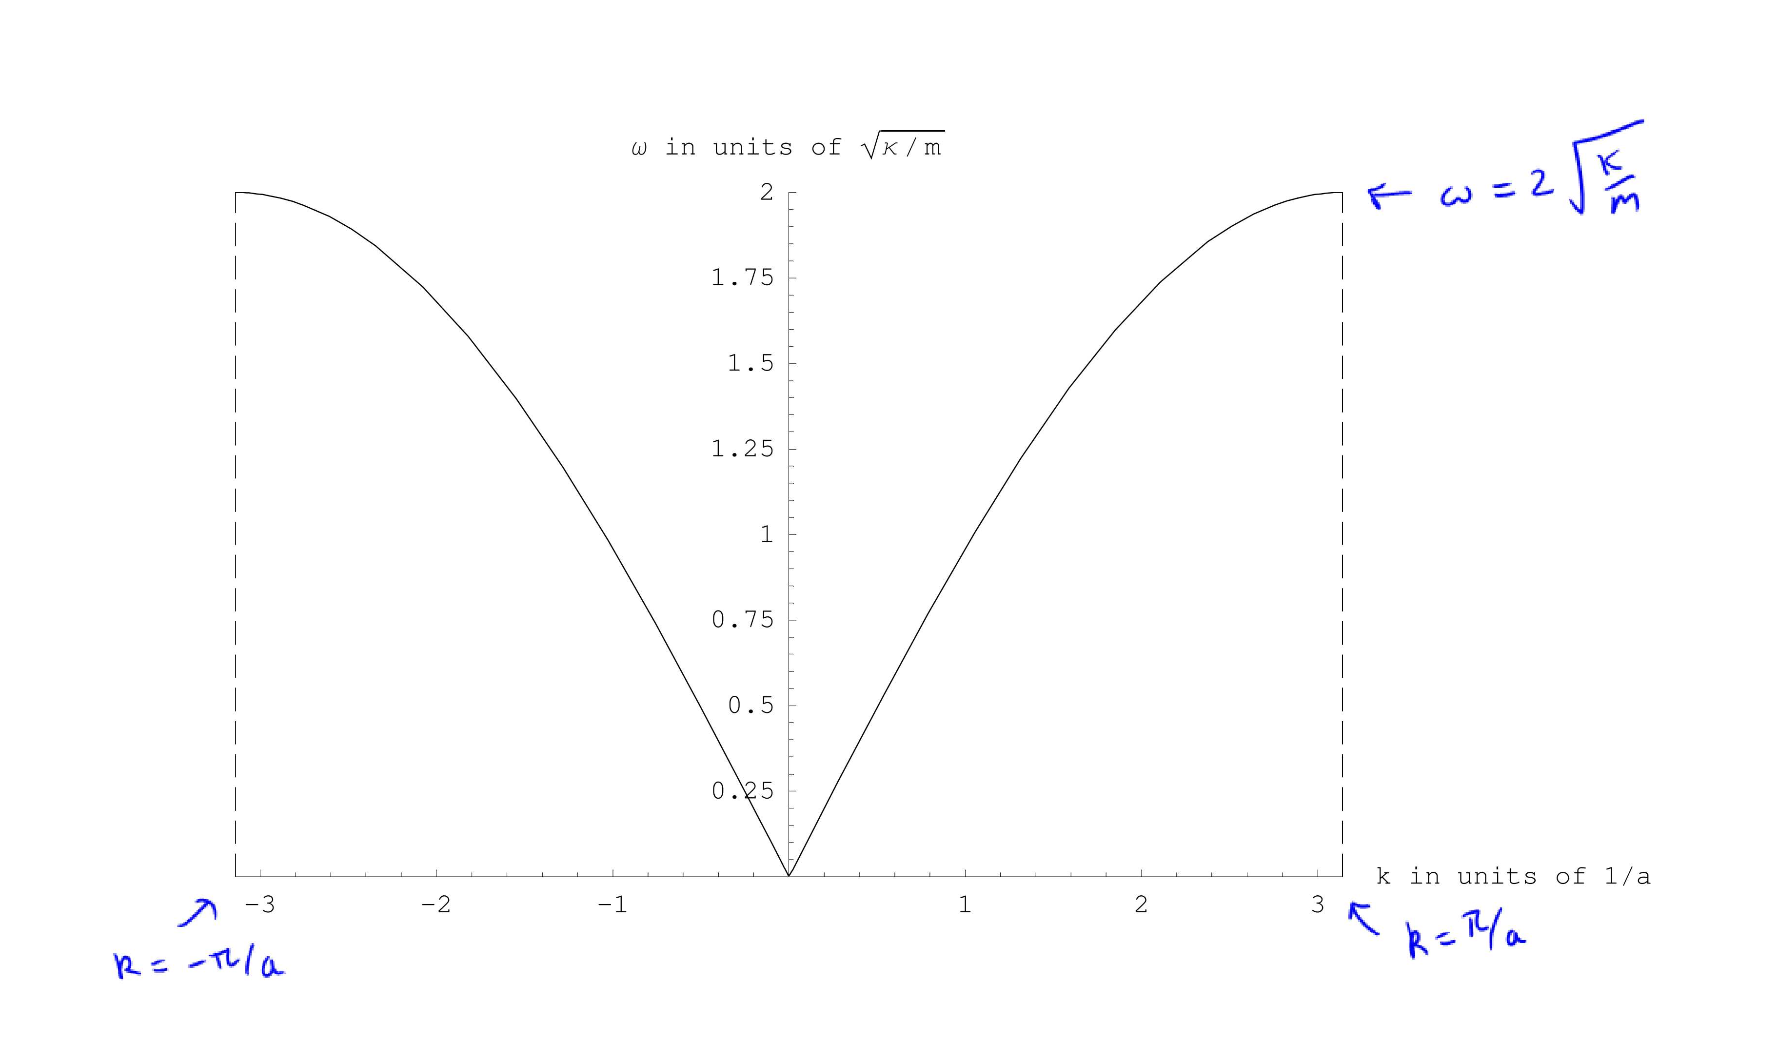
\includegraphics[width=\linewidth]{1d_disp.png}
  \caption{Dispersion relation for 1D monatomic chain.}
\end{figure}

\subsection{Reciprocal Lattice}
The dispersion relation in Fig. 1 is periodic in $k \rightarrow k + 2\pi/a$. An important
general principle is the following: \emph{A system which is periodic in real space with a periodicity
$a$ will be periodic in reciprocal space with periodicity $2\pi/a$}. In other words, if the system "looks
the same" when $x \rightarrow x + a$, then the dispersion will look the same when $k \rightarrow k + 2\pi/a$.


The periodic unit in $k$-space is known as the \emph{Brillouin zone}. The \emph{first Brillouin zone} is centered about $k = 0$.
The points $k = \pm \pi/a$  in Fig. 1 are known as the \emph{Brillouin zone boundary}.


If we take $k \rightarrow k + 2\pi p/a$, where $p$ is any integer, then our solution for $\delta x_{n}$ will not change since it is
a deep fact that
$$e^{i2\pi n p} = 1$$
The \emph{reciprocal lattice} is therefore defined as a set of point in $k$-space (\emph{reciprocal space}) which are physically
equivalent to the point $k = 0$. The set of points $x_{n}$ are known as the \emph{direct lattice} or \emph{real-space lattice}.

As an example, the points in the direct lattice of the one-dimensional monatomic chain with lattice spacing $a$ are
$$x_{n} = ..., -2a, -a, 0, a, 2a, ...$$
and the reciprocal lattice points are
$$G_{n} = ..., -2\left (\frac{2\pi}{a} \right), -\left (\frac{2\pi}{a} \right), 0, \left (\frac{2\pi}{a} \right), 2\left (\frac{2\pi}{a} \right),... $$
And the defining property of the reciprocal lattice points are:
\begin{equation}
  \boxed{e^{iG_{m}x_{n}} = 1}
\end{equation}
That is, a point $G_{m}$ is in the reciprocal lattice only if the above holds for all $x_{n}$ in the direct lattice.
An important note: $k$ and $k+G_{m}$ only describe the same wave when measured at direct lattice points $x_{n}$. If measured arbitrarily
along the x-axis, they may differ.

\subsection{Sound Waves}
Sound waves are vibrations with a long wavelength compared to the interatomic spacing. That is, $k = \frac{2\pi}{\lambda}$, where $\lambda >> a$.
Therefore, the dispersion becomes
$$\omega = v_{sound}k = \left ( a \sqrt{\frac{\kappa}{m}}\right)k$$
At larger $k$ (shorter $\lambda$), the dispersion is no longer linear and one typically defines two velocities.
\begin{itemize}
  \item The group velocity $v_{group} = d\omega /dk$. The speed at which the wavepacket moves. The group velocity becomes 0 at the Brillouin zone boundary.
  \item The phase velocity $v_{phase} = \omega / k$. The speed at which individual minima/maxima move.
\end{itemize}

\subsection{Counting Normal Modes}
At first glance, it would appear that any choice of $k$ in the first Brillouin zone yields a unique normal mode with frequency $\omega(k)$.
But periodic boundary conditions imply that $x_{n} = x_{n + N}$. This yields the requirement in our solution that
$$e^{ikNa} = 1$$
From which we obtain the restriction on possible values of $k$:
$$k = \frac{2\pi m}{Na}$$
where $m$ is some integer. So the full dispersion relation only contain several allowed $k$ values, the spacing between which is $2\pi/Na$.
The total number of normal modes is therefore given by the range of the Brillouin zone (e.g. $[-\pi/a,\pi/a]$), divided by the spacing between
allowed normal mode values of $k$. Be careful to only include one endpoint in the Brillouin zone.

\subsection{Quantum Phonons}
Quantum correspondance: If a classical harmonic system has a normal oscillation mode at frequency $\omega$ the corresponding
quantum system will have eigenstates with energy
$$E_{n} = \hbar \omega (n + \frac{1}{2})$$
\begin{itemize}
\item At a given wavevector $k$ there are many possible eigenstates.
\item The ground state is the $n = 0$ state with zero point energy $\hbar \omega(k)/2$.
\item All excitations occur in units of $\hbar \omega(k)$.
\end{itemize}
A \emph{phonon} is a discrete quantum of vibration, and corresponds to an excitation of the normal mode by increasing the
quantum number $n$.
\begin{itemize}
  \item Phonons are bosons. We may think of them as particles with energy $\hbar \omega$ and \emph{crystal} momentum $\hbar k$. We always describe
  momentum using $k$ within the first Brillouin zone. Even though $k$ is equivalent to $k + G_{m}$, they do not describe the same momentum.
  \item At finite temperature, there are non-zero number of phonons occupying a given mode, described by the Bose occupation factor:
  $$n_{B}(\beta \hbar \omega) = \frac{1}{e^{\beta \hbar \omega} - 1}$$
  \item The expectation value of energy of phonons at wavevector $k$ is given by
  $$E_{k} = \hbar \omega(k) \left (n_{B}(\beta \hbar \omega) + \frac{1}{2} \right )$$
  \item The total energy is given by
  $$U_{tot} = \sum_{k} E_{k}$$
  where the sum is over all possible normal modes (i.e. $\frac{-\pi}{a} < k \leq \frac{\pi}{a}$, such that $k = \frac{2\pi m}{Na}$).
  When the system is very large, the spacing between normal modes shrinks, and we may convert the sum into an integral.
  $$\sum_{k} \rightarrow \frac{Na}{2\pi}\int_{-\pi/a}^{\pi/a}dk$$.
  \item We also note that the total number of normal modes is given by
  $$\frac{Na}{2\pi}\int_{-\pi/a}^{\pi/a}dk$$
  \item From the integral form of $U_{tot}$, we could calculate the heat capacity
  $$C = \frac{dU}{dT}$$
  \item This approach is identical to the Debye model, except that Debye assumed $\omega = vk$, whereas our dispersion
  relation is much more complicated.
  \item We may also convert the integral over $k$ to an integral over $\omega$ by introducing a density of states $g(\omega)$.
  $$\frac{Na}{2\pi}\int_{-\pi/a}^{\pi/a}dk = \int d\omega g(\omega)$$
  $$g(\omega) = 2 \frac{Na}{2\pi}\left | \frac{dk}{d\omega}\right |$$
\end{itemize}

\section{Vibrations of the One-Dimensional Diatomic Chain}
Consider a one-dimensional chain of alternating masses $m_{1}$ and $m_{2}$ with alternating connecting spring constants $\kappa_{1}$ and $\kappa_{2}$.
The unit cell for the diatomic chain consists of both masses and is of length (lattice constant) $a$. It is useful to pick a reference point for each unit
cell, the set of these reference points forms a simple lattice. Within each unit cell, the individual atoms in the cell are described relative to the reference
point - this description forms the basis.

\subsection{Normal Modes}
Assume for now that $m_{1} = m_{2} = m$. The equations of motion follow from the monatomic case. But now, let $x_{n}$ be the position of the $n$th $m_{1}$
mass and $y_{n}$ be the position of the $n$th $m_{2}$ mass. Let $\kappa_{1}$ connect $y_{n}$ to $x_{n+1}$.
$$m\ddot{\delta x_{n}} = \kappa_{2}(\delta y_{n} - \delta x_{n}) + \kappa_{1}(\delta y_{n-1} - \delta x_{n})$$
$$m\ddot{\delta y_{n}} = \kappa_{1}(\delta x_{n+1} - \delta y_{n}) + \kappa_{2}(\delta x_{n} - \delta y_{n})$$
The ansatz solutions will be
$$\delta x_{n} = A_{x}e^{i \omega t - ikna}$$
$$\delta y_{n} = A_{y}e^{i \omega t - ikna}$$
\begin{itemize}
  \item Because the lattice spacing is $a$, $k$ is physically equivalent to $2\pi/a$, so the first Brillouin zone is defined by
  $$-\pi/a \geq k \leq \pi/a$$
  \item For $N$ unit cells, such that the system length is $L = Na$, the allowed values of $k$ are
  $$k = \frac{2\pi m}{Na} = \frac{2 \pi m}{L}$$
  \item The number of possible $k$ values is $N$ - one value of $k$ per unit cell.
  \item Debye's intuition: there should be one mode per degree of freedom. We have $2N$ degrees of freedom, but $N$ values of $k$. Resolution:
  there are two modes per $k$ value.
\end{itemize}

Plugging in the ansatz solutions to the equations of motion yields
$$-\omega^{2}mA_{x} = \kappa_{2}A_{y} + \kappa_{1}A_{y}e^{ika} - (\kappa_{1} + \kappa_{2})A_{x}$$
$$-\omega^{2}mA_{y} = \kappa_{1}A_{x}e^{-ika} + \kappa_{2}A_{x} - (\kappa_{1} + \kappa_{2})A_{y}$$

This can be written as
$$
m\omega^{2} \begin{bmatrix}
A_{x}\\ A_{y}
\end{bmatrix} =
\begin{bmatrix}
 (\kappa_{1} + \kappa_{2})& -\kappa_{2} - \kappa_{1}e^{ika}\\
-\kappa_{2}-\kappa_{1}e^{-ika} & (\kappa_{1} + \kappa_{2})
\end{bmatrix}
\begin{bmatrix}
A_{x}\\ A_{y}
\end{bmatrix}
$$

The solutions are obtained by finding the zeroes of the characteristic determinant.
$$
0 = \begin{vmatrix}
 (\kappa_{1} + \kappa_{2}) - m\omega^{2}& -\kappa_{2} - \kappa_{1}e^{ika}\\
-\kappa_{2}-\kappa_{1}e^{-ika} & (\kappa_{1} + \kappa_{2})-m\omega^{2}
\end{vmatrix}
$$

The roots are given by
$$
m\omega^{2} = (\kappa_{1} + \kappa_{2}) \pm \left | \kappa_{1} + \kappa_{2}e^{ika}\right |
$$
which can be written as
$$
\omega^{2} = \frac{(\kappa_{1} + \kappa_{2})}{m} \pm \frac{\sqrt{\kappa_{1}^{2} + \kappa_{2}^{2} + 2\kappa_{1}\kappa_{2}cos(ka)}}{m}
$$
The $\pm$ in the dispersion indicates that there are two branches of the dispersion for each $k$ value - and therefore $2N$ normal modes
in total.

\begin{figure}
  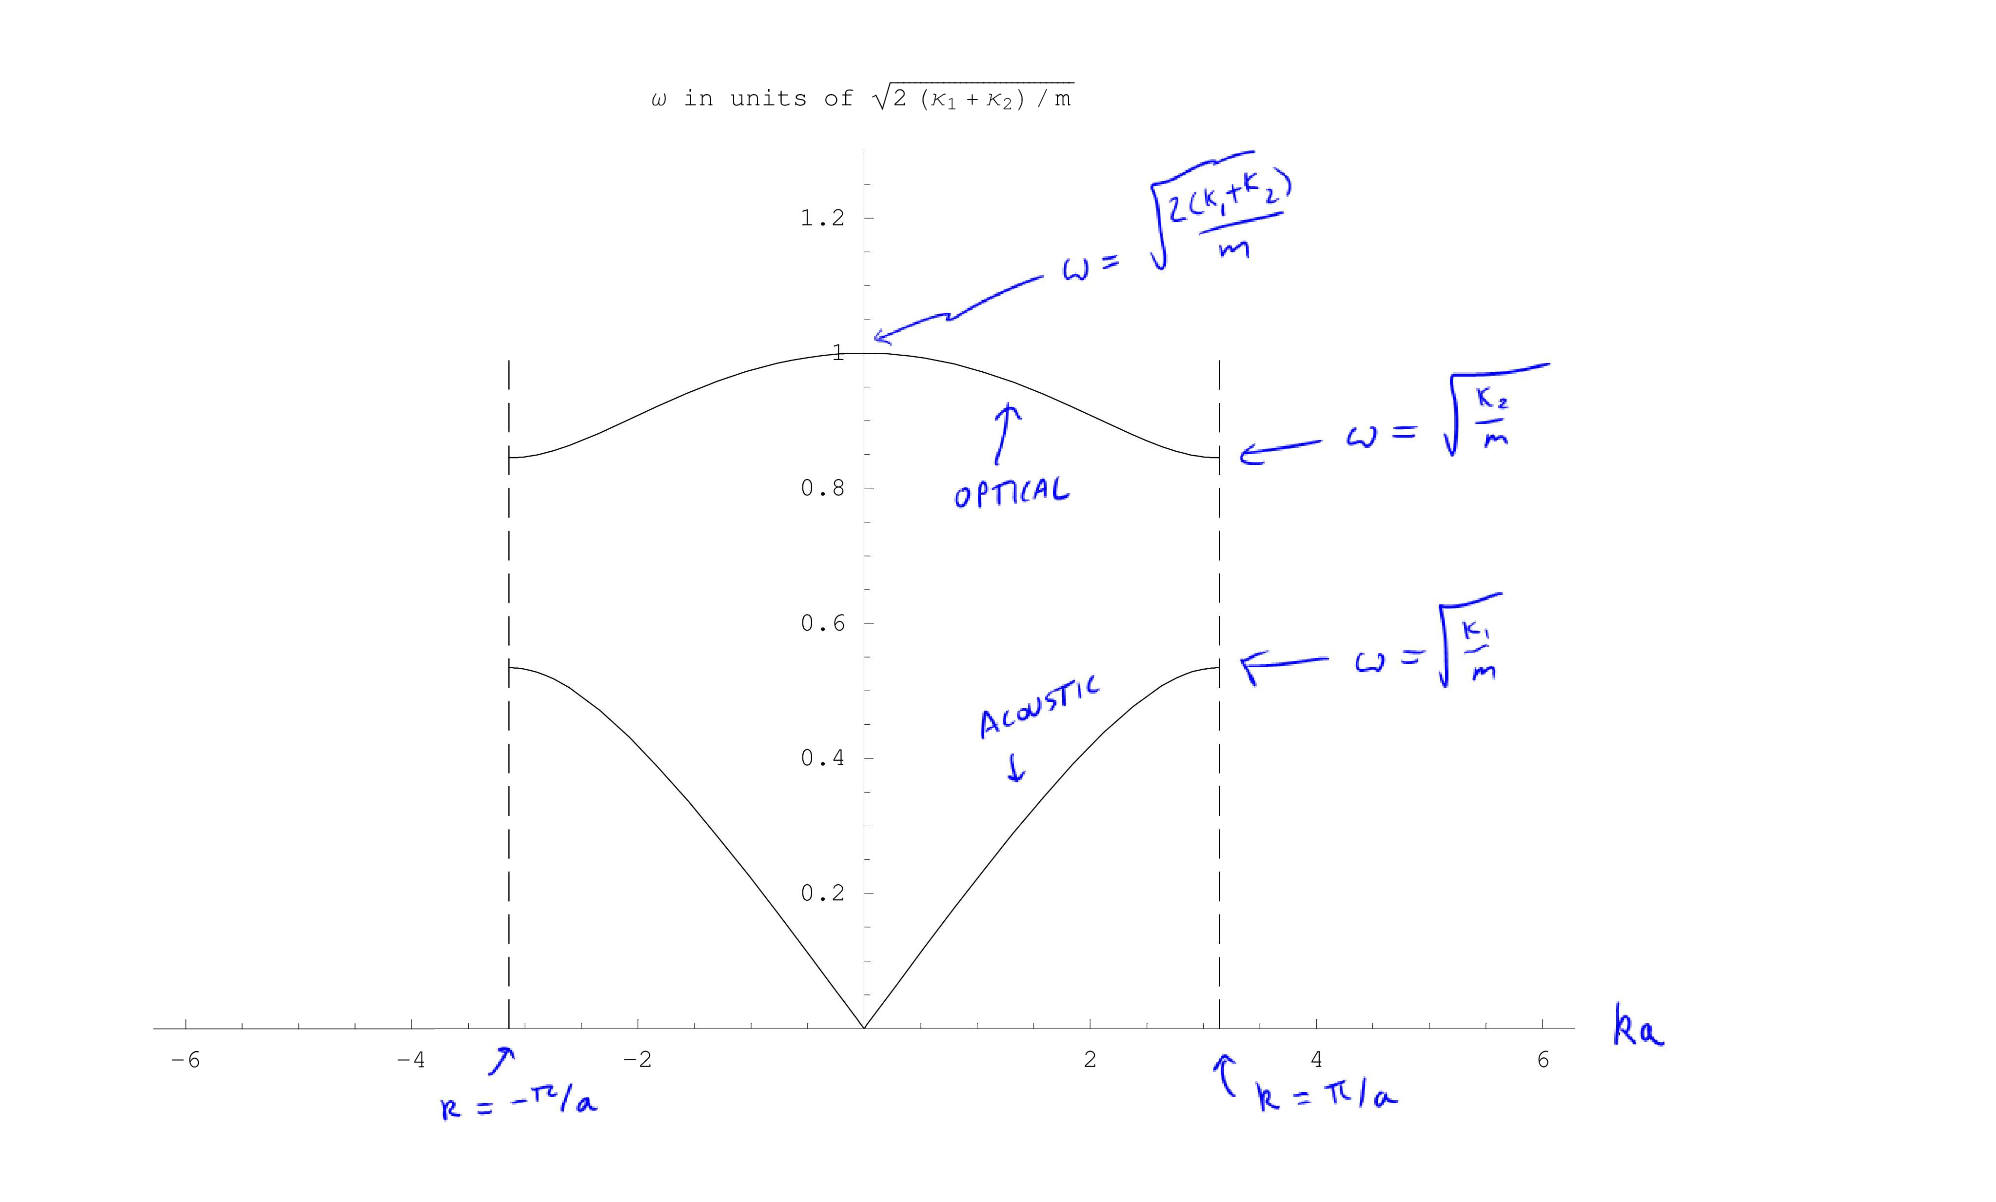
\includegraphics[width=\linewidth]{1d_dia_disp.png}
  \caption{Dispersion relation for 1D diatomic chain.}
\end{figure}

The long-wavelength, low-energy branch of excitations with linear dispersion (corresponding to $\omega_{-}$ as $k \rightarrow 0$) is the
\emph{acoustic mode}. In this linear region, we expect
$$\omega_{-} = v_{sound}k$$
Therefore,
$$v_{sound} = \frac{d\omega_{-}}{dk} = \sqrt{\frac{a^{2}\kappa_{1}\kappa_{2}}{2m(\kappa_{1}+\kappa_{2})}}$$

The higher-energy branch is the \emph{optical mode}. At $k = 0$, the optical frequency is
$$\omega_{+}(k = 0) = \sqrt{\frac{2(\kappa_{1} + \kappa_{2})}{m}}$$
and $v_{group} = \omega_{+}' = 0$. Side note: optical modes are so-named because photons can only be absorbed by solids for very small $k$ (since
photon energy is given by $\omega = ck$). But at very small $k$, only the optical modes have enough energy to absorb a photon and conserve energy.

\subsubsection{The Long Wavelength Limit}
In the long wavelength limit ($k \rightarrow 0$), the eigenvalue equation becomes
$$
\omega^{2} \begin{bmatrix}
A_{x}\\ A_{y}
\end{bmatrix} = \frac{\kappa_{1} + \kappa_{2}}{m}
\begin{bmatrix}
 1 & -1 \\
-1 & 1
\end{bmatrix}
\begin{bmatrix}
A_{x}\\ A_{y}
\end{bmatrix}
$$

\begin{itemize}
  \item As $k \rightarrow 0$, $\omega_{-} \rightarrow 0$, and we obtain
  $$A_{x} = A_{y} = 1$$
  which indicates that the two masses in the unit cell move together (in-phase) in the long wavelength limit
  of the acoustic mode.
  \item As $k \rightarrow 0$, $\omega_{+}^{2} \rightarrow \frac{2(\kappa_{1} + \kappa_{2})}{m}$, and we obtain
  $$A_{x} = -A_{y}$$
  which indicates that the two masses in the unit cell move in opposite directions ($180$ degrees out of phase) in
  the long wavelength limit of the optical mode.
\end{itemize}

Note: in the case of $M$ atoms per unit cell, there will be $M$ modes per distinct value of $k$ (i.e. $M$ dispersion branches) and one branch
will be acoustic ($w(k) \rightarrow 0$ as $k \rightarrow 0$) while the rest are optical. When higher degrees of freedom (e.g. transverse motion)
are allowed, we must take them into account when determining number of modes. For example, 3D crystals with $n$ atoms per unit cell have $3n$ degrees of
freedom per unit cell and $3n$ total dispersion branches - $3$ of these are acoustic, while $3(n-1)$ are optical.

\subsubsection{The Brillouin Zone Boundary}
At the Brillouin zone boundary, $k = \pm \frac{\pi}{a}$. The frequencies are (assuming $\kappa_{1} > \kappa_{2}$)
$$
\omega_{-} = \sqrt{\frac{2\kappa_{2}}{m}}
$$
$$
\omega_{+} =  \sqrt{\frac{2\kappa_{1}}{m}}
$$
and, in both cases, $v_{group} \rightarrow 0$.

\subsection{Brillouin Zone Schemes and Monoatomic Perturbations }
\begin{itemize}
  \item The \emph{reduced zone scheme} is the plotting of all dispersion relations within the first Brillouin zone only. See Fig. 2.
  \item The \emph{extended zone scheme} is the plotting of all dispersion relations across multiple Brillouin zones such that each $k$
  point is mapped to a single mode. See Fig. 3.
\end{itemize}

In the limit $\kappa_{1} \rightarrow \kappa_{2}$, the two atoms in the unit cell become truly indistinguishable and we approach the simple monatomic
chain situation with lattice constant $a/2$. We can see that the dispersion curve of the diatomic chain with lattice constant $a$ will also approach that of a monatomic chain
with lattice constant $a/2$ (see Fig. 4).
\begin{figure}
  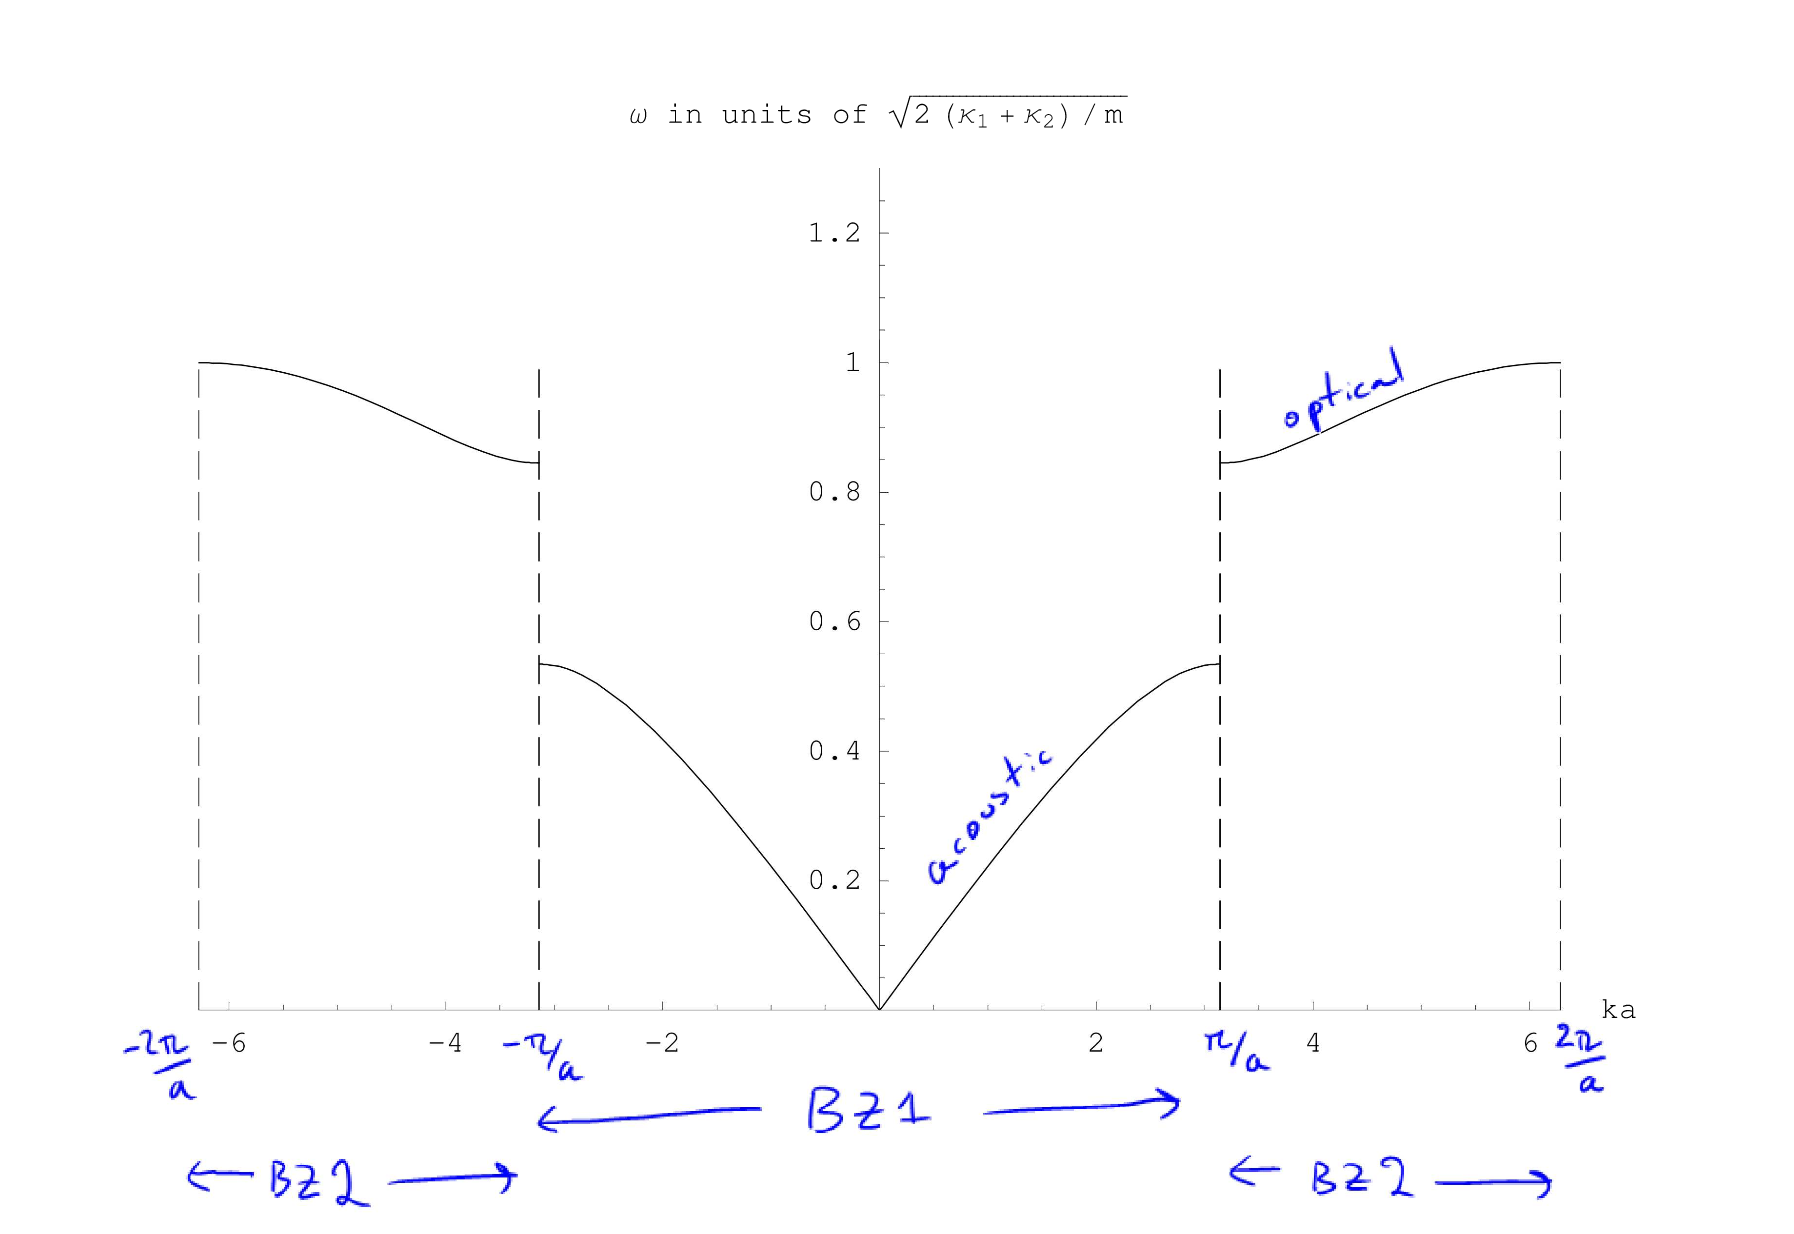
\includegraphics[width=\linewidth]{1d_dia_ext.png}
  \caption{Dispersion relation for 1D diatomic chain.}
\end{figure}

\begin{figure}
  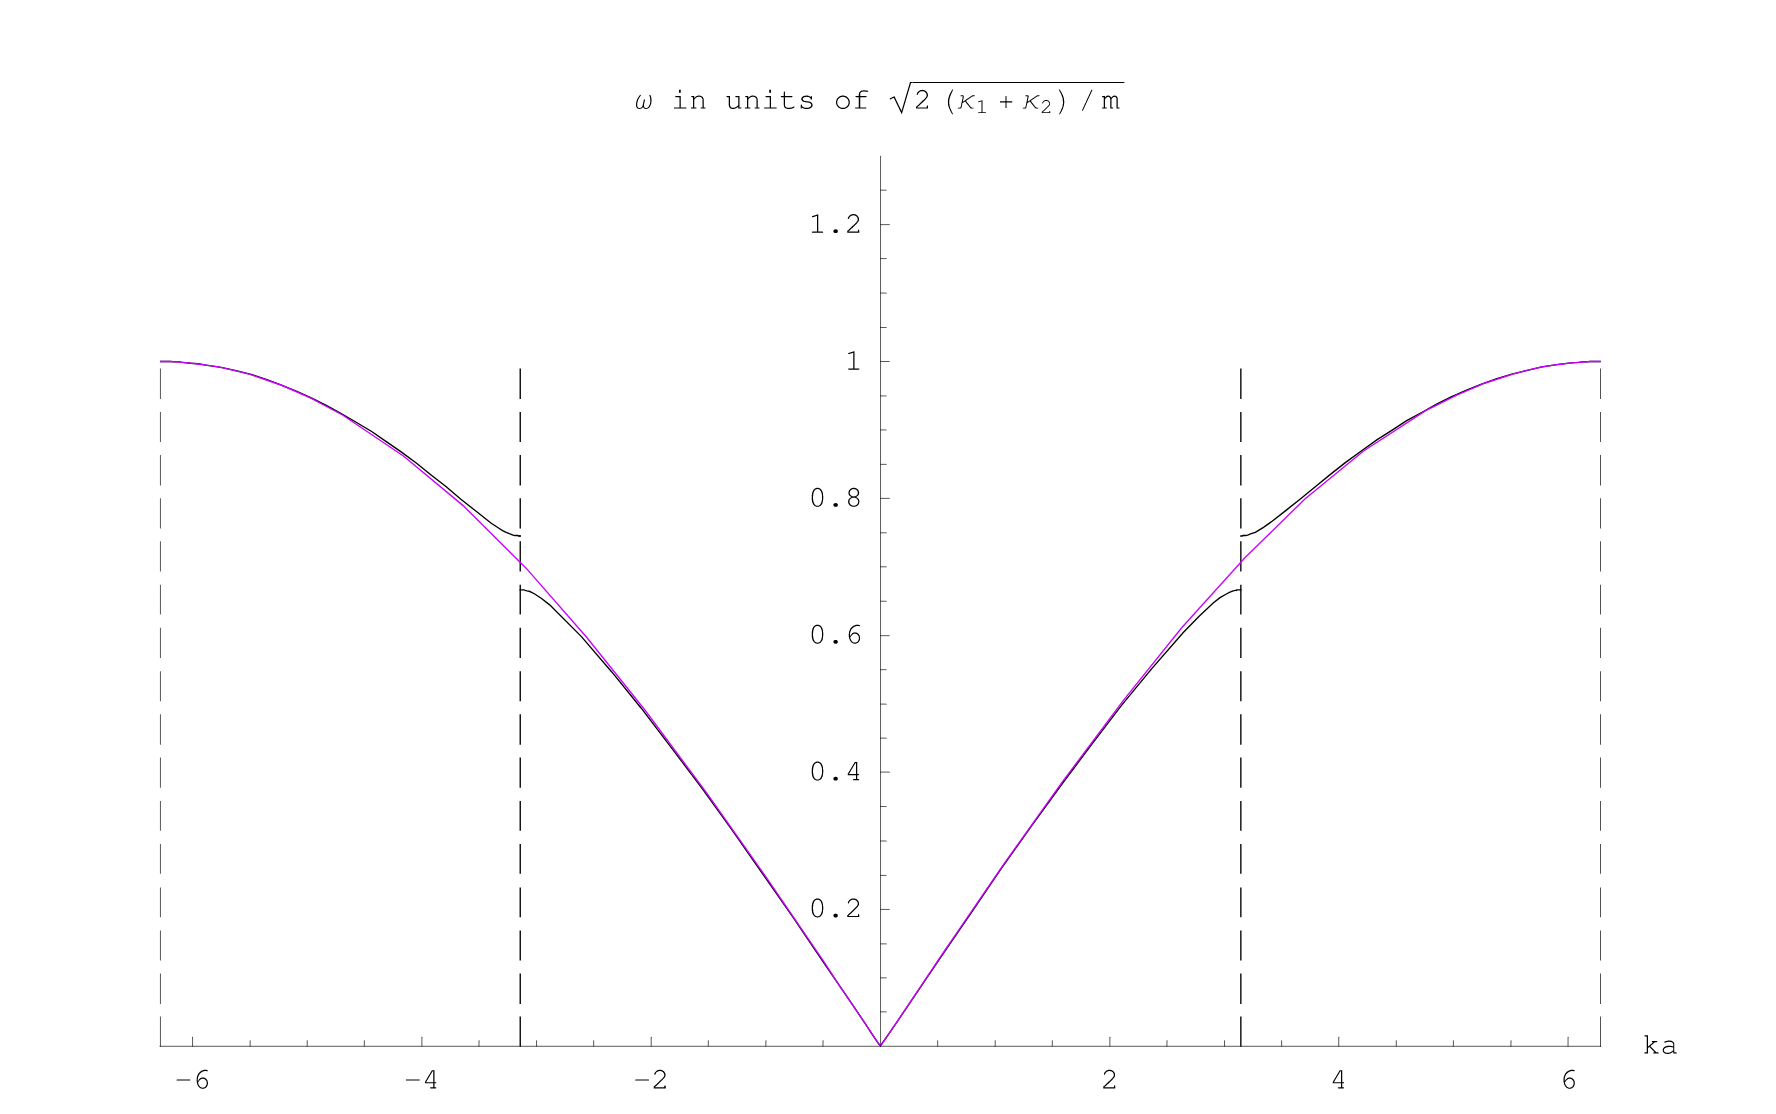
\includegraphics[width=\linewidth]{1d_dia_to_mono.png}
  \caption{Dispersion relation for 1D diatomic chain as $\kappa_{1} \rightarrow \kappa_{2}$.}
\end{figure}

When the atoms in the unit cell are slightly different, a small gap opens at the Brillouin zone boundary, but the dispersion will continue to mostly
look like the monatomic case.


\section{Crystal Structure}
\subsection{Basics of Crystal Structure}
\begin{itemize}
\item A \emph{lattice} is an infinite set of points defined by integer sums of a set of linearly
independent \emph{primitive lattice vectors}.
\item Alternatively: A \emph{lattice} is an infintie discrete set of vectors where addition of
any two vectors in the set gives a third vector in the set, or a \emph{lattice} is an infinite
discrete set of points where the environment of any given point is equivalent to the environment
of any other point.
\item Lattice points may be described in three dimensions as
$$\textbf{R} = n_{1}\textbf{a}_{1} + n_{2}\textbf{a}_2 + n_{3}\textbf{a}_{3}$$
\item In 2+ dimensions, the choice of primitice lattice vectors is not unique.
\end{itemize}

\begin{itemize}
  \item A \emph{unit cell} is the repeated motif which is the elementary building block of
  any periodic structure. When many identical unit cells are tiled together, they
  completely fill all of space and reconstruct the full structure.
  \item A \emph{primitive unit cell} is a unit cell containing exactly one lattice point.
  \item A \emph{conventional unit cell} is a typically less-minimal unit cell, often
  with orthogonal axes, chosen due to ease of use.
  \item A \emph{Wigner-Seitz cell} is constructed by including all points in space that are
  closer to a given lattice point than any other lattice point. Approach: choose a lattice cell
  and draw lines to all possible neighbors. Perpendicular bisectors of these lines bound the
  Wigner-Seitz cell.
  \item The description of the unit cell with respect to the associated lattice point is
  known as the \emph{basis}.
  \item The positions of atoms can be described by
  $$ \textbf{R} = \textbf{R}_{lattice} + \textbf{R}_{basis} $$
  \item The \emph{coordination number} of a lattice is the number of nearest neighbors to any point of the lattice.
\end{itemize}

\subsection{Three-Dimensional Lattices}
The simplest example is the \emph{simple cubic} lattice.
\begin{itemize}
  \item The primitive unit cell is typically a cube, where each corner contributes $1/8$ lattice point.
  \item \emph{Tetragonal} and \emph{orthorhombic} lattices have two and three different primitive lattice
  vector lengths, respectively.
  \item A point in the lattice may be written as $[uvw]$ where
  $$[uvw] =  u\textbf{a}_{1} + v\textbf{a}_2 + w\textbf{a}_{3}$$
  \item In the case of orthogonal axes, $\textbf{a}_{1}$ is assumed to be in the $\hat{x}$ direction, etc.
\end{itemize}

The \emph{body-centered cubic} lattice is identical to the simple cubic lattice, but with an additional
lattice point in the center of the cube.
\begin{itemize}
  \item The conventional unit cell contains $8(1/8) + 1 = 2$ lattice points.
  \item The points of the BCC lattice can be written as
  $$\textbf{R}_{corner} = [n_{1}, n_{2}, n_{3}]$$
  $$\textbf{R}_{center} = [n_{1}, n_{2}, n_{3}] + [1/2, 1/2, 1/2]$$
  \item We can also think of the BCC as two interpenetrating SC lattices, displaced by $[1/2, 1/2, 1/2]$.
  \item The coordination number $Z = 8$.
  \item One choice of primitive lattice vectors:
  $$\textbf{a}_{1} = [1, 0, 0]$$
  $$\textbf{a}_{2} = [0, 1, 0]$$
  $$\textbf{a}_{3} = [1/2, 1/2, 1/2]$$

\end{itemize}

The \emph{face-centered cubic} lattice is similar to the simple cubic lattice, but with the addition of a
lattice point on every cube face.
\begin{itemize}
\item The conventional unit cell contains $8(1/8) + 6(1/2) = 4$ lattice points.
\item The points of the FCC lattice can be written as
$$\textbf{R}_{corner} = [n_{1}, n_{2}, n_{3}]$$
$$\textbf{R}_{xy} = [n_{1}, n_{2}, n_{3}] + [1/2, 1/2, 0]$$
$$\textbf{R}_{yz} = [n_{1}, n_{2}, n_{3}] + [0, 1/2, 1/2]$$
$$\textbf{R}_{zx} = [n_{1}, n_{2}, n_{3}] + [1/2, 0, 1/2]$$
\item We can also think of the FCC as four interpenetrating SC lattices, displaced as described above.
\item One choice of primitive lattice vectors:
$$\textbf{a}_{1} = [1/2, 1/2, 0]$$
$$\textbf{a}_{2} = [1/2, 0, 1/2]$$
$$\textbf{a}_{3} = [0, 1/2, 1/2]$$
\end{itemize}

\section{Reciprocal Lattice, Brillouin Zone, Waves in Crystals}

\subsection{General Reciprocal Lattice Definition}
Given a direct lattice of points $\textbf{R}$, a point $\textbf{G}$ is a point in the reciprocal lattice if and only if
\begin{equation}
  \boxed{e^{i\textbf{G}\cdot \textbf{R}} = 1}
\end{equation}
for all points $\textbf{R}$ of the direct lattice. If we write the points of the direct lattice in the form
$$
\textbf{R} = n_{1}\textbf{a}_{1} + n_{2}\textbf{a}_{2} + n_{3}\textbf{a}_{3}
$$
where $\textbf{a}_{i}$ are the primitive lattice vectors, then the points of the reciprocal lattice can be written in
the form
$$
\textbf{G} = m_{1}\textbf{b}_{1} + m_{2}\textbf{b}_{2} + m_{3}\textbf{b}_{3}
$$
where $\textbf{b}_{i}$ are the primitive reciprocal lattice vectors and $$\textbf{a}_{i}\cdot\textbf{b}_{j} = 2\pi \delta_{ij}$$.


Note: one such choice of $\textbf{b}_{i}$ is
$$
\textbf{b}_{1} = \frac{2\pi \textbf{a}_{2} \times \textbf{a}_{3}}{\textbf{a}_{1} \cdot (\textbf{a}_{2} \times \textbf{a}_{3})}
$$
$$
\textbf{b}_{2} = \frac{2\pi \textbf{a}_{3} \times \textbf{a}_{1}}{\textbf{a}_{1} \cdot (\textbf{a}_{2} \times \textbf{a}_{3})}
$$
$$
\textbf{b}_{3} = \frac{2\pi \textbf{a}_{1} \times \textbf{a}_{2}}{\textbf{a}_{1} \cdot (\textbf{a}_{2} \times \textbf{a}_{3})}
$$

\subsection{Reciprocal Lattice as a Fourier Transform}
In one-dimension, the direct lattice is given by $R_{n} = an$. The density could then be written as
$$\rho(r) = \sum_{n}\delta(r - an)$$
The Fourier tranform is then
$$\mathcal{F}[\rho(r)] = \int dr e^{ikr} \rho(r) = \sum_{n} \int dr e^{ikr} \delta(r-an) = \sum_{n}e^{ikan}$$
Since $e^{ikan} = 1$ if $k = 2\pi m/a$ (that is, if $k$ is a point on the reciprocal lattice) the sum will accumulate infinitely. If $k$ does not meet this condition, the sum terms
will oscillate and converge to 0. We obtain
$$\mathcal{F}[\rho(r)] = \sum_{n}e^{ikan} = \frac{2\pi}{|a|}\sum_{m}\delta(k - 2 \pi m/ a)$$

In higher dimensions, with $v$ the volume of the unit cell,

$$\mathcal{F}[\rho(\textbf{r})] = \sum_{\textbf{R}} e^{i\textbf{k}\cdot\textbf{R}} = \frac{(2\pi)^{D}}{v} \sum_{\textbf{G}} \delta^{D}(\textbf{k} - \textbf{G})$$

\subsubsection{Fourier transform of any periodic function}
For any periodic function $\rho(\textbf{r})$ where $\rho(\textbf{r}) = \rho(\textbf{r} + \textbf{R})$ for any lattice vector $\textbf{R}$, the
Fourier transform is written
$$\mathcal{F}[\rho(\textbf{r})] = \int d^3 r e^{i\textbf{k}\cdot\textbf{r}}\rho(\textbf{r})$$
We can break up the integral over all space into a sum of integrals over unit cells.
$$\mathcal{F}[\rho(\textbf{r})] = \sum_{\textbf{R}}\int_{unit-cell} d^3 x e^{i\textbf{k}\cdot(\textbf{R}+\textbf{x})}\rho(\textbf{R} + \textbf{x})$$
Since $\textbf{x}$ is equivalent to $\textbf{x} + \textbf{R}$,
$$\mathcal{F}[\rho(\textbf{r})] = \sum_{\textbf{R}}e^{i\textbf{k}\cdot\textbf{R}}\int_{unit-cell} d^3 x e^{i\textbf{k}\cdot\textbf{x}}\rho(\textbf{x})$$
$$\mathcal{F}[\rho(\textbf{r})] = \frac{(2\pi)^{D}}{v} \sum_{\textbf{G}} \delta^{D}(\textbf{k} - \textbf{G}) \cdot \textbf{R}S(\textbf{k})$$
where the structure factor $S(\textbf{k})$ is given by
$$S(\textbf{k}) = \int_{unit-cell} d^3 x e^{i\textbf{k}\cdot\textbf{x}}\rho(\textbf{x})$$

\subsection{Reciprocal Lattice Points as Families of Lattice Planes}
\begin{itemize}
\item A \emph{lattice plane} or \emph{crystal plane} is a plane containing at least three non-collinear points of a lattice.
\item A family of lattice planes is an infinite set of equally-spaced parallel lattice planes containing every point in the lattice.
\item The families of lattice planes are in one-to-one correspondance with the possible directions of reciprocal lattice vectors, to which
they are normal. Further, the spacing between these lattice planes is $d = 2\pi/|\textbf{G}_{min}|$ where $\textbf{G}_{min}$ is the minimum
length reciprocal lattice vector in this normal direction.
\item The relationship $\textbf{G}\cdot \textbf{r} = 2\pi m$, where $\textbf{r}$ is a set of points defining a plane, defines a set of
lattice planes (each with a different value of $m$). Not every plane needs to contain a lattice point, but the distance between planes is necessarily
$d = 2\pi/|\textbf{G}|$. The minimal set of planes that capture all lattice points are defined by a maximal spacing $d = 2\pi/|\textbf{G}_{min}|$.
\end{itemize}

\subsubsection{Miller indices}
Miller indices can be used to denote a reciprocal lattice vector, and therefore a family of lattice planes.
\begin{itemize}
  \item One first chooses edge vectors for the direct unit cell, $\textbf{a}_{i}$.
  \item Then construct $\textbf{b}_{i}$ such that $\textbf{a}_{i}\cdot \textbf{b}_{j} = 2\pi\delta_{ij}$.
  \item Reciprocal space vector $\textbf{G}$ may then be written as
  $$G_{(h,k,l)} = h\textbf{b}_{1} + k\textbf{b}_{2} + l\textbf{b}_{3}$$
  \item If $\textbf{a}_{i}$ are primitive, so too will be $\textbf{b}_{i}$. Then, any set of indices $(hkl)$ will represent a reciprocal
  space lattice vector. To represent a family of planes, $(hkl)$ should be chosen to have no common divisor - if they do, they represent a family
  of planes that do not all necessarily contain direct lattice points.
  \item If $\textbf{a}_{i}$ are non-primitive, then neither will be $\textbf{b}_{i}$. In this case, not all combinations of $(hkl)$ are reciprocal lattice vectors.
  \item The spacing between adjacent planes is given by
  $$ d = \frac{2\pi}{|\textbf{G}|} = \frac{2\pi}{\sqrt{h^{2}|\textbf{b}_{1}|^{2} + k^{2}|\textbf{b}_{2}|^{2} + l^{2}|\textbf{b}_{3}|^{2}}}$$
  where $\textbf{b}_{i}$ are assumed orthogonal and so $|b_{i}| = 2\pi/|a_{i}|$. Therefore,
  $$\frac{1}{|d_{(hkl)}|^{2}} = \frac{h^2}{a_{1}^2} + \frac{k^2}{a_{2}^2} + \frac{l^2}{a_{3}^2}$$
  \item The Miller indices may be obtained by examining the intercepts on the coordinate axis. The relationship is:
  $$
  \frac{1}{x_{1}}:\frac{1}{x_{2}}:\frac{1}{x_{3}} = h:k:l
  $$
  Then $(hkl)$ should be scaled such that they represent the smallest set of integers with this ratio.

\subsection{General Brillouin Zone}
The \emph{Brillouin zone}, in general, is any primitive unit cell of the reciprocal lattice.
\begin{itemize}
  \item Physical waves in crystals are unchanged if their wavevector is shifted by a reciprocal lattice vector $\textbf{k} \rightarrow \textbf{k} + \textbf{G}$.
  \item The Brillouin zone contains every physically inequivalent crystal momentum, and they all appear exactly once.
  \item Construction: start with $\textbf{G} = 0$. All $\textbf{k}$ points closer to 0 than any other reciprocal lattice vector constitute the first
  Brillouin zone. All $\textbf{k}$ points for which $\textbf{G} = 0$ is the second-closest reciprocal lattice point constitute the second Brillouin zone, etc.
  \item Draw lines connecting the point $\textbf{G} = 0$ to all reciprocal space points. Draw perpendicular bisectors across these lines. Any point that can be
  reached without crossing a bisector is in the first Brillouin zone. Any point that can be reached by only crossing one bisector is in the second Brillouin zone, etc.
  \item Higher Brillouin zones are necessarily made of disconnected pieces.
  \item On the Brillouin zone boundary, between 0 and $\textbf{G}$, lies a point that is physically equivalent to the point found by adding $-\textbf{G}$ to this point.
  \item Every Brillouin zone has the same total area. There are exactly as many $k$ states within a Brillouin zone as there are unit cells in system.
\end{itemize}

\end{itemize}
\section{Misc}
\begin{itemize}
  \item $$\sin(x) = \frac{e^{ix} - e^{-ix}}{2i}$$
  \item $$\cos(x) = \frac{e^{ix} + e^{-ix}}{2}$$
  \item $$\sin^{2}(x) = \frac{1 - \cos(2x)}{2}$$
  \item $$\cos^{2}(x) = \frac{1 + \cos(2x)}{2}$$
\end{itemize}
\end{document}
